\apendice{Manual del programador.} % usar el término que mejor se corresponda.

\section{Estructura de directorios}
El código fuente desarrollado a lo largo de este proyecto se encuentra estructurado y accesible a través de diferentes repositorios de \textit{GitHub} \cite{github}, separados de acuerdo a las tres arquitecturas propuestas: el entorno de producción hospitalario, el terminal portátil (\textit{Raspberry Pi}) y el entorno de desarrollo local. 

No obstante, con el objetivo de facilitar la comprensión y el análisis técnico del trabajo, en este apartado se detallará exclusivamente la estructura y el contenido de los ficheros correspondientes al \textbf{despliegue local con la base de datos integrada mediante \textit{Docker}}: \href{https://github.com/ngg1017/TFG-2026-Nicolas-Garcia-Gomez}{TFG-2026-Nicolas-Garcia-Gomez}. Se ha seleccionado esta versión como referencia principal para la memoria dado que engloba la totalidad de la lógica de negocio, las herramientas de migración y el entorno completo de pruebas del sistema.

\begin{itemize}
	\item \texttt{README.md}\\Pequeña introducción y explicación sobre el trabajo y los recursos disponibles en el repositorio.
	
	\item \texttt{LICENCE}\\Documento de la licencia \textit{Apache License 2.0} utilizada para este proyecto.
	
	\item \texttt{.gitignore}\\Documento de configuración que le indica a \textit{Git} qué archivos o carpetas (como los documentos \textit{CSV} con datos médicos sensibles o el entorno virtual) debe ignorar por completo para no subirlos nunca a tu repositorio de \textit{GitHub}.
	
	\item \texttt{requirements.txt}\\Listado que contiene todas las librerías externas que necesita el proyecto para funcionar.
	
	\item \texttt{rxconfig.py}\\Documento de configuración central del \textit{framework Reflex}, encargado de definir los parámetros globales de la aplicación, como su nombre, el puerto de ejecución o las conexiones, para que el sistema arranque con los ajustes correctos.
	
	\item \texttt{.env} \\Archivo de configuración segura que almacena las variables de entorno y credenciales sensibles (como usuarios, contraseñas y la \textit{URL} de conexión a la base de datos), separándolas del código fuente por motivos de seguridad.
	
	\item \texttt{.dockerignore} \\Archivo de exclusión que indica a \textit{Docker} qué directorios locales (como \textit{cachés}, entornos virtuales o archivos ocultos) deben omitirse al construir la imagen, optimizando así el peso final del contenedor.
	
	\item \texttt{Dockerfile} \\Documento de texto que contiene todas las instrucciones secuenciales para construir la imagen del entorno de la aplicación (define el sistema operativo base, instala las dependencias de \textit{Python} y ejecuta el servidor de \textit{Reflex}).
	
	\item \texttt{docker-compose.yml} \\Archivo de orquestación en formato \textit{YAML} que define y coordina la arquitectura completa del sistema. Levanta simultáneamente los servicios (\textit{frontend}/\textit{backend} y base de datos), estableciendo sus puertos, redes internas y volúmenes de persistencia.
	
	\item \texttt{alembic.ini} \\Es el archivo de configuración principal de la herramienta de migraciones. Actúa como el centro de mando que le indica a \textit{Alembic} dónde está la carpeta con los historiales, qué formato usar para generar los nuevos archivos y cómo debe comportarse al conectarse. Es básicamente el manual de instrucciones inicial para que el sistema de migraciones sepa cómo arrancar y trabajar con el proyecto.
	
	\item \texttt{alembic/.} \\Es el corazón de las migraciones. Cada vez que se cambie algo en el código y se ejecute el comando \texttt{makemigrations}, aquí se genera un nuevo archivo \textit{Python}. Estos archivos son los ``planos de obra'' secuenciales que contienen las instrucciones matemáticas exactas (ej. ``crear tabla paciente'', ``añadir columna edad'') que \textit{PostgreSQL} debe ejecutar para actualizarse sin perder los datos clínicos que ya tiene guardados.
	
	\item \texttt{Datos/.}\\Contiene todos los archivos utilizados para las demostraciones y pruebas de la aplicación.
		\begin{itemize}
			\item \texttt{Datos\_2016\_2025.csv}\\Conjuntos de archivos \textit{CSV} sintéticos utilizados para el desarrollo de la \textit{web}
			
			\item \texttt{Datos.txt}\\Archivos de texto que describe todos los datos a recoger y sus tipos en la unidad.
			
			\item \texttt{importador.py}\\\textit{Script} administrativo independiente diseñado para automatizar el proceso \textit{ETL} (Extracción, Transformación y Carga), permitiendo limpiar, normalizar y migrar de forma masiva los historiales clínicos desde archivos \textit{CSV} a la base de datos \textit{PostgreSQL}.
		\end{itemize}
		
	\item \texttt{Documentacion\_Latex/.}\\Carpeta que contiene todos los archivos empleados en el desarrollo de
la memoria. Incluye los documentos pdf de la memoria y anexos.
		\begin{itemize}
			\item \texttt{/img/.}\\Localización de todas las imágenes empleadas tanto en la memoria como en los anexos.
			\item \texttt{/tex/.}\\Carpeta que almacena todos los capítulos de la memoria y anexos en sus respectivos documentos \textit{LaTeX}.
		\end{itemize}
		
	\item \texttt{Logica/.}\\Almacena todos los archivos de \textit{Python}(\textit{.py}) necesarios para el correcto funcionamiento del \textit{Backend}.
		\begin{itemize}
			\item \texttt{BBDD.py}\\Archivo que administra la lógica relacionada con la base de datos. Contiene las funciones que administran la carga de registros, así como su edición, modificación y visualización en pantalla.
			
			\item \texttt{Modelo.py}\\Define los modelos que estructuran las tablas de la base de datos para almacenar los historiales clínicos, registrar los \textit{logs} de auditoría y gestionar las credenciales de los usuarios.
			
			\item \texttt{PDF.py}\\Archivo que contiene toda la lógica relativa al procesamiento del informe final. Recibe todos los datos y gráficas calculadas y se encarga de su correcta colocación.
			
			\item \texttt{Programa.py}\\Contiene la gran mayoría del procesamiento y cálculo de indicadores. Recibe los registros en la \textit{RAM} cargados por el usuario y realiza la computación de todos los indicadores, el resumen, y la mezcla.
			
			\item \texttt{State.py}\\Se encarga de la recepción de los archivos y el control de la lista \textit{FIFO}. Controla que el máximo de años almacenados sea de diez y que el formato sea el admitido por la herramienta. Además almacena todos los métodos de borrado.
			
			\item \texttt{Usuarios.py}\\Constituye el núcleo de seguridad y control de acceso de la aplicación web. Se encarga de gestionar de forma íntegra la autenticación de los usuarios mediante cifrado unidireccional (\textit{Bcrypt}), la validación de credenciales frente a la base de datos y la administración de los diferentes roles y permisos.
		\end{itemize}
			
	\item \texttt{TFG\_2026\_Nicolas\_Garcia\_Gomez/.}\\Directorio que almacena todos los componentes relativos al \textit{frontend}, por que en todos ellos se utiliza código de \textit{Reflex}.
		\begin{itemize}
			\item \texttt{TFG\_2026\_Nicolas\_Garcia\_Gomez.py}\\Funciona como el módulo orquestador. Su única responsabilidad es instanciar el objeto \texttt{rx.App}, definir el árbol de navegación (rutas) e importar los diferentes componentes modulares de la interfaz para compilarlos.
			\item \texttt{constantes.py}\\Contiene \textit{URL} constantes de las diferentes referencias y \textit{links} utilizados en la \textit{web}.
			\item \texttt{/componentes/.}\\Contiene todos los diferentes componentes gráficos utilizados en la herramienta.
				\begin{itemize}
					\item \texttt{boton\_subida.py}\\Archivo que despliega el botón de subida.
					\item \texttt{graficos.py}\\Archivo que contiene todos los gráfico utilizados en \textit{Reflex}.
					\item \texttt{link\_icon.py}\\Contiene un botón interactivo para el uso de enlaces externos.
					\item \texttt{mezcla.py}\\Archivo que se utiliza para el despliegue del método mezcla. Al tener tantos componente visuales diferentes al resto de indicadores se separó por limpieza y pulcritud.
					\item \texttt{renderizar\_campo\_formulario.py}\\Define una función que genera visualmente un campo de formulario dinámico, adaptando automáticamente el tipo de control (desplegable \textit{booleano}, entrada de fecha, número o texto) y su diseño según la categoría a la que pertenezca el dato.
					\item \texttt{seleccion.py}\\Fichero que almacena todos los componentes visuales del menú desplegable de indicadores. Además controla la llamada a cada uno de los método una vez seleccionado la opción deseada.
					\item \texttt{tabla.py}\\Registro que contiene todos los componentes para la creación de tablas. En un inicio se encontraba en el archivo \texttt{vent\_flotante.py} separándose por limpieza.
				\end{itemize}
			
			\item \texttt{/estilos/.}\\Carpeta que contiene todos los archivo relacionados a la fuente, colores y estilado de la \textit{web}.
				\begin{itemize}
					\item \texttt{colores.py}\\Almacena los colores como enumerados (\textit{Enum}).
					\item \texttt{estilos.py}\\Contiene tamaños estándar utilizados, hojas de estilo \cite{roboto_estilo} \cite{bootstrap} y el estilo base para la \textit{web}.
					\item \texttt{fuentes.py}\\Contiene la fuente utilizada \textit{Roboto} \cite{roboto}.
					
					\item \texttt{Roboto-Regular.ttf}\\Archivo con la fuente \textit{Roboto} utilizada en el informe \textit{PDF} para utilizar caracteres especiales.
				\end{itemize}
				
				
			\item \texttt{/views/.}\\Directorio, el cual contiene todas las vistas y partes de la página.
				\begin{itemize}
					\item \texttt{acceso.py}\\Contiene los tres componente gráficos de la validación de usuarios. El inicio de sesión, el cambio de contraseña y el panel de gestión para los administradores.
					\item \texttt{cabecera.py}\\Almacena la primera parte de la página donde se da la bienvenida al usuario y se dan las diferentes instrucciones de uso.
					\item \texttt{instrucciones.py}\\Parte de la \textit{web} que contiene las instrucciones de su funcionamiento, así como el botón de subida y el disparados del menú de selección de indicadores.
					\item \texttt{navbar.py}\\Componente que muestra la barra fija superior, donde se encuentra el enlace a la página de la \textit{URCCPQ} y el título de la \textit{web}.
					\item \texttt{pie.py}\\Muestra el pie de la página, conteniendo el nombre del autor y el escudo de la \textit{UBU}.
					
					\item \texttt{vent\_flotante.py}\\Componente principal de la herramienta. Se almacena toda la lógica que permite mostrar diferentes componentes para cada opción del menú multiselección. Por ejemplo: a través de condicionales en \textit{Reflex} (\texttt{rx.cond}) este componente es capaz de mostrar los indicadores individuales con sus tarjetas (\texttt{rx.card}) de datos o mostrar las tablas del resumen.
					
					\item \texttt{vistas\_bbdd.py}\\Despliega toda la lógica de visualización de la interfaz de la \textit{BBDD}. Muestra u oculta las diferentes funcionalidades que permite la base de datos en función del rol del usuario.
				\end{itemize}
		\end{itemize}	
	
	\item \texttt{assets/.}\\Directorio que contiene todas las imágenes y el icono de la \textit{web}.
		\begin{itemize}
			\item \texttt{favicon.ico}\\Icono de la \textit{web} con el logo del \textit{SaCyl}.
			\item \texttt{urccpq.png}\\Imagen de la unidad.
			\item \texttt{sacyl.png}\\Logo del \textit{SaCyl}.
			\item \texttt{ubu.png}\\Logo de la Universidad de Burgos \textit{UBU}.
		\end{itemize}
\end{itemize}

\section{Pruebas del sistema} \label{sec:Practica}
La validación de la plataforma clínica trasciende la mera comprobación de la interfaz gráfica. El plan de pruebas se ha diseñado bajo un enfoque de \textit{Defensive Programming} (Programación Defensiva), asumiendo por defecto que las entradas del usuario o de las fuentes externas pueden contener errores de formato, omisiones o inconsistencias lógicas. A continuación, se detallan los bloques de pruebas críticas realizados, abarcando desde el despliegue del entorno hasta la validación transaccional de los datos médicos.

\subsection{Despliegue de Infraestructura y Puesta en Marcha}
El primer nivel de pruebas garantiza que el sistema es reproducible y puede ser desplegado de manera consistente en cualquier equipo u hospital, simulando las condiciones de la \textit{intranet} clínica.

\begin{itemize}
    \item \textbf{Objetivo de la prueba:} Verificar la correcta construcción de los contenedores \textit{Docker} a partir del repositorio de código, la inicialización de la base de datos y la aplicación automática de las migraciones estructurales, se proporciona un vídeo que explica todo el proceso descrito en este apartado: \textbf{\href{https://youtu.be/eCAgFDYIzCw}{Primer Arranque de la Herramienta}}.
    \item \textbf{Ejecución y Resultado:} 
    \begin{enumerate}
    		\item \textbf{Instalación de los requisitos previos:} Antes de operar con el código fuente, el equipo anfitrión debe contar con las herramientas base para la gestión de versiones y la contenerización. Se requiere la descarga e instalación de \href{https://www.docker.com/}{\textit{Docker Desktop}}.
    			\begin{itemize}
    				\item \textbf{Nota importante para entornos \textit{Windows}:} Para garantizar el correcto arranque del motor de \textit{Docker}, es indispensable verificar que la virtualización por \textit{hardware} se encuentre habilitada en la configuración de la \textit{BIOS} del equipo. Asimismo, se requiere que el Subsistema de \textit{Windows} para \textit{Linux} (\textit{\href{https://learn.microsoft.com/es-es/windows/wsl/install}{\textit{WSL 2}}}) esté correctamente instalado y configurado. En caso de presentar errores de inicialización, se recomienda ejecutar los comandos de actualización del núcleo en la terminal (\texttt{wsl -{}-install} o \texttt{wsl -{}-update}) y reiniciar el sistema.
    			\end{itemize}
        \item \textbf{Obtención del código fuente:} Es necesario obtener el código de la aplicación eligiendo entre las dos siguientes vías: 
        	\begin{itemize}
        		\item Se debe abrir una terminal o consola de comandos, navegar hasta el directorio de destino deseado y clonar el repositorio del proyecto ejecutando la siguiente instrucción: \texttt{git clone https://github.com/ngg1017/TFG-2026-Nicolas-Garcia-Gomez}.
        		
        		\item Descargarlo directamente desde el el repositorio \textit{online} \cite{github}
        	\end{itemize}
        	
        	\item \textbf{Configuración de las variables de entorno:} Por motivos de seguridad y buenas prácticas de desarrollo (definidas en los archivos \texttt{.gitignore} y \texttt{.dockerignore}), las credenciales sensibles no se deben de incluyen en el repositorio público. En este proyecto se ha decidido subir un archivo \texttt{.env} a modo de ejemplo directamente a \textit{GitHub} para facilitar la configuración incial. Si se desea se puede editar el archivo de texto plano (\texttt{.env}) facilitado. Este archivo debe contener la cadena de conexión a la base de datos, siguiendo este formato: \texttt{DATABASE\_URL=postgresql://medico:secreto123@db\_hospital:5432/hospital\_db}
        	
        	\item \textbf{Construcción y levantamiento de la infraestructura:} Una vez configuradas las credenciales, se ordena a \textit{Docker} la construcción de las imágenes y el despliegue de los servicios (el servidor \textit{web} y el motor de base de datos) en segundo plano. Para ello, se ejecuta: \texttt{docker-compose up -{}-build -d} en el directorio raíz. En la imagen \ref{fig:compose} se muestra el resultado de la consola de este primer comando.
        	
        	\begin{figure}[hbt!]
    			\centering
    			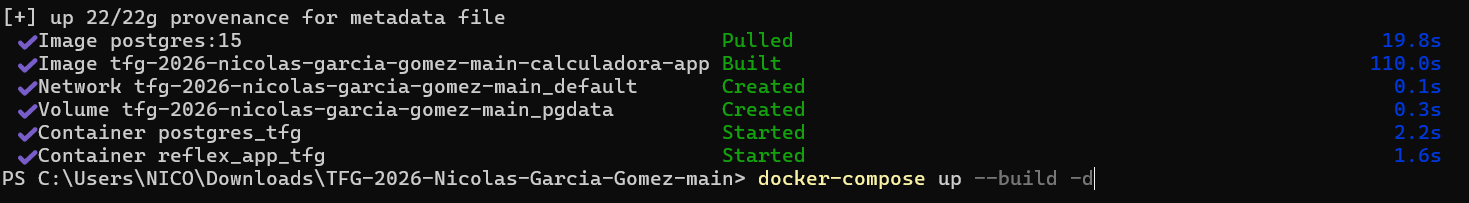
\includegraphics[width=1\textwidth]{img/compose.png}
    			\caption{Trazas de consola confirmando la creación de las imágenes}
    			\label{fig:compose}
		\end{figure}
        
        \item \textbf{Migración de la estructura de la base de datos:} Tras el levantamiento de los contenedores, el gestor de base de datos se encuentra vacío. Para que la herramienta \textit{Alembic} traduzca los modelos de datos implementados en \textit{Python} a sentencias \textit{DDL} y construya la estructura de tablas y columnas correspondientes, se debe ejecutar la orden \texttt{docker exec reflex\_app\_tfg reflex db migrate}, si este comando no devuelve ningún tipo de log como se muestra en la imagen \ref{fig:migracion} se puede pasar al siguiente punto o dar por finalizada la configuración.
        
        	\begin{figure}[hbt!]
    			\centering
    			
\includegraphics[width=1\textwidth]{img/migracion.png}
    			\caption{Consola ejecutando la migración exitosa de la base de datos.}
    			\label{fig:migracion}
		\end{figure} 
    
		\item \textbf{Carga inicial de datos históricos (Opcional):} Si se requiere que la aplicación parta con información previa, se procederá a ejecutar el \textit{script} administrativo encargado del proceso de \textbf{Extracción, Transformación y Carga (\textit{ETL})}. Este volcará los registros de los archivos locales a la base de datos recién creada. En la figura \ref{fig:importacion} se muestra el proceso completo.
			\begin{itemize}
				\item La primera parte de este volcado consiste en activar \textit{Python} o algún entorno virtual disponible.
				\item Posteriormente se hace un desplazamiento mediante el comando \textit{cd} a la carpeta \textbf{Datos}.
				\item Finalmente se ejecuta el \textit{scrip} de importación cargando la \textit{BBDD} con una serie de registro generados aleatoriamente para la prueba de la herramienta.
			\end{itemize}
			
		\begin{figure}[hbt!]
    			\centering
    			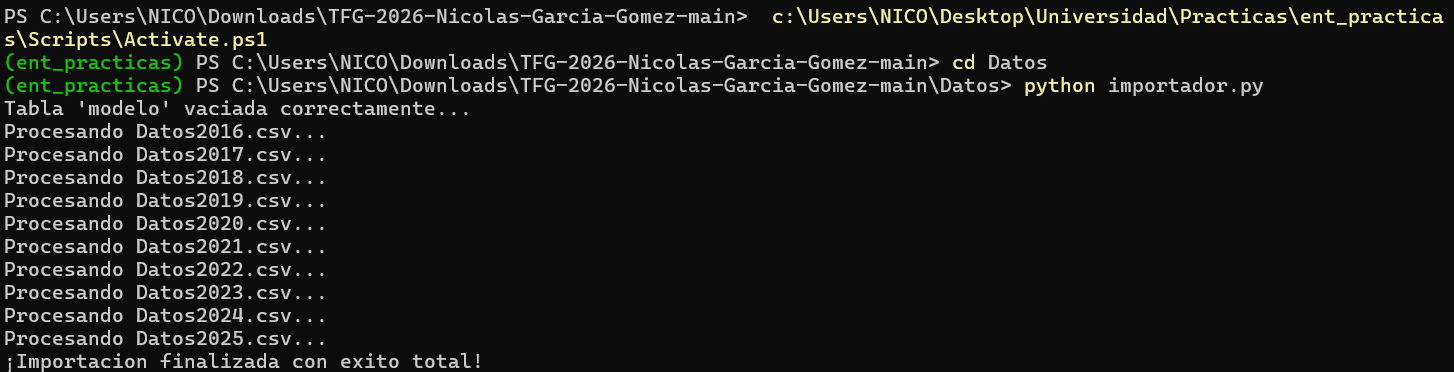
\includegraphics[width=1\textwidth]{img/importacion.png}
    			\caption{Consola mostrando todos los pasos necesarios para la importación de los registros iniciales.}
    			\label{fig:importacion}
		\end{figure}
		
		\item \textbf{Comprobación de acceso local:} Una vez finalizados los pasos anteriores, la aplicación estará completamente operativa. Se puede verificar su funcionamiento accediendo a través del navegador web del equipo anfitrión a la dirección: \texttt{http://localhost:3000}.
        
    \end{enumerate}
\end{itemize}

\subsection{Gestión del Ciclo de Vida del Servidor}
Una vez realizada la instalación y el primer despliegue, no es necesario repetir los pasos descritos anteriormente. El encendido y apagado rutinario del sistema se puede gestionar de dos formas equivalentes:

\begin{enumerate}
	\item \textbf{Apagado Rutinario (Uso Diario Recomendado):} Para pausar el servidor al final de la jornada laboral sin destruir la infraestructura, se recomienda utilizar el apagado en suspensión. Los contenedores quedan ``dormidos'' y listos para arrancar inmediatamente al día siguiente: 
	\begin{itemize}
		\item Ejecutar el comando \texttt{docker-compose stop} para detener el servicio, y \texttt{docker-compose start} para reanudarlo. El resultado de la consola de ambos comandos se refleja en la siguiente imagen \ref{fig:inicio_comandos}.
		
		\begin{figure}[hbt!]
    			\centering
    			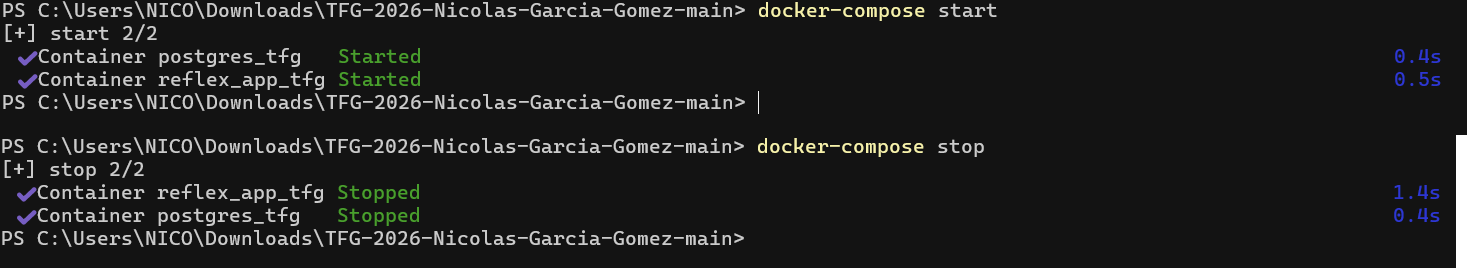
\includegraphics[width=1\textwidth]{img/inicio_comandos.png}
    			\caption{Consola mostrando el arranque y detención correcto.}
    			\label{fig:inicio_comandos}
		\end{figure}
		
		\item \textbf{Mediante interfaz gráfica (GUI):} Abriendo la aplicación \textit{Docker Desktop}, ubicando el contenedor correspondiente al proyecto en la pestaña \textit{Containers} y utilizando los botones de acción integrados (\textit{Play} para arrancar y \textit{Stop} para detener). En la siguiente imagen se muestran ambos botones \ref{fig:inicio_docker}.
		
		\begin{figure}[hbt!]
    			\centering
    			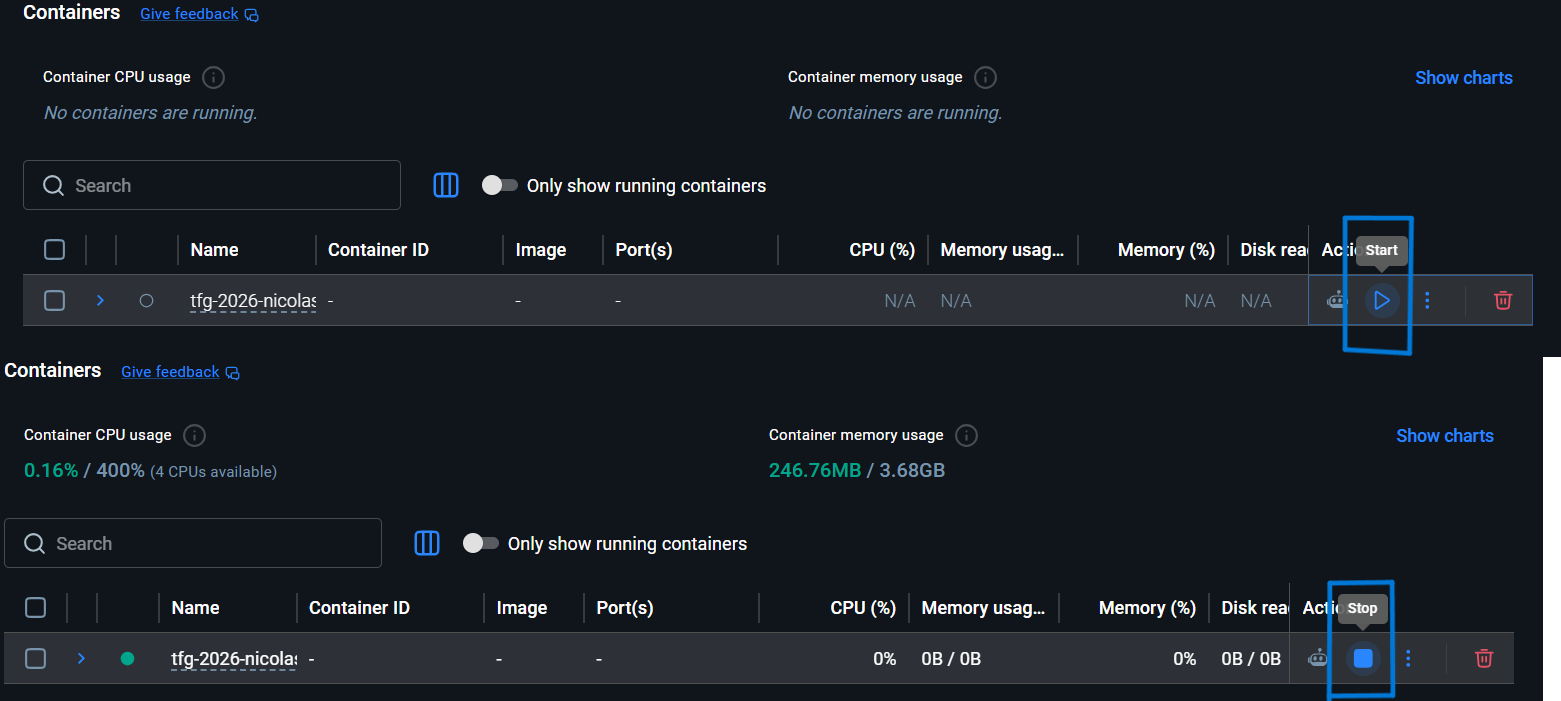
\includegraphics[width=1\textwidth]{img/inicio_docker.png}
    			\caption{Botones en la interfaz de \textit{Docker Desktop}.}
    			\label{fig:inicio_docker}
		\end{figure}
		
	\end{itemize}
	
	\item \textbf{Apagado de Mantenimiento (Destrucción de Contenedores):} Si se necesita hacer una limpieza profunda del sistema, liberar memoria en el servidor o aplicar actualizaciones estructurales, se debe proceder a la destrucción de los contenedores actuales (los datos clínicos de los pacientes no se pierden, ya que están blindados en un volumen persistente). En la siguiente imagen se muestra la destrucción y el reinicio \ref{fig:inicio_terminal}.
	\begin{itemize}
		\item Ejecutar el comando: \texttt{docker-compose down}.
		\item Al usar este comando, para volver a encender el servidor será necesario ejecutar \texttt{docker-compose up -d} para que el sistema vuelva a construir los contenedores a partir de los datos guardados.
	\end{itemize}
	
	\begin{figure}[hbt!]
    		\centering
    		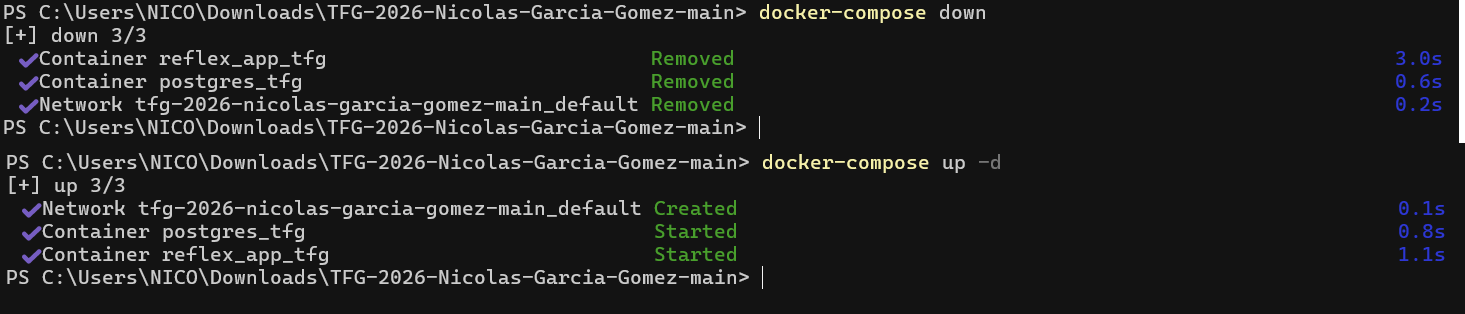
\includegraphics[width=1\textwidth]{img/inicio_terminal.png}
    		\caption{Borrado y reinicio del los contenedores.}
    		\label{fig:inicio_terminal}
	\end{figure}
	
	
\end{enumerate}

\subsection{Acceso Remoto mediante Red Local (LAN)}
La arquitectura de red del proyecto permite que la aplicación actúe como un nodo centralizado, posibilitando el acceso desde cualquier dispositivo externo (como pueden ser otros ordenadores, \textit{tablets} o dispositivos móviles del personal médico) que se encuentre conectado a la misma red local que el servidor principal. Para establecer esta conexión:

\begin{enumerate}
	\item Se debe identificar la dirección \textit{IPv4} local del equipo que aloja el servidor (ejecutando el comando \texttt{ipconfig} en la terminal de \textit{Windows}, o \texttt{ifconfig} en sistemas \textit{Unix/Linux}).
	
	\item En el navegador web de cualquier dispositivo cliente de la red, se introducirá dicha dirección \textit{IP} seguida del puerto de exposición de la aplicación. Suponiendo, a modo de ejemplo, que la \textit{IP} del servidor sea \texttt{192.168.1.45}, el acceso se realizará a través de la URL: \texttt{http://192.168.1.45:3000}.
	
Cabe destacar que, debido a las políticas de seguridad restrictivas de los sistemas operativos modernos (basadas en arquitecturas \textit{Zero Trust}), el cortafuegos o \textit{firewall} del equipo anfitrión bloquea por defecto cualquier intento de conexión entrante que no utilice puertos estándar. Por consiguiente, si no se realiza una configuración adicional, los dispositivos cliente de la red local obtendrán un error de tiempo de espera (\textit{timeout}) al intentar acceder a la dirección \textit{IP} del servidor.

Para que el acceso a la herramienta sea efectivo, resulta indispensable configurar el perímetro de seguridad del nodo principal. En el siguiente vídeo \textbf{\href{https://youtu.be/zeIvf4545cU}{Configuración \textit{Firewall}}}, se documenta paso a paso la resolución técnica de este bloqueo, ilustrando el procedimiento necesario para transformar un entorno local hermético en un servidor accesible.

En la demostración práctica se detalla la configuración del \textit{Firewall} de \textit{Windows} con seguridad avanzada, donde se establece una nueva \textbf{Regla de Entrada}. Esta directiva se configura para autorizar explícitamente el tráfico de red bajo el protocolo \textit{TCP} dirigido al puerto local \texttt{3000}. Esta apertura perimetral, específica y controlada, es el requisito fundamental que habilita la comunicación bidireccional segura entre los dispositivos del hospital y el contenedor \textit{Docker} que aloja la aplicación principal.	
\end{enumerate}


\subsection{Control de Ingesta Volátil (Archivos \textit{CSV})}
Para el análisis de sesiones clínicas aisladas, el sistema permite la carga de archivos exportados. Para evitar el desbordamiento de memoria y asegurar el rendimiento, se implementan políticas estrictas de restricción.

\subsubsection{Control de Ingesta: Restricción de Formato y Gestión \textit{FIFO}}
Dadas las limitaciones visuales, de almacenamiento y de procesamiento del terminal portátil o equipo de la \textit{URCCPQ}, el sistema implementa una política estricta de gestión de archivos para evitar el desbordamiento de memoria y asegurar el rendimiento.

\begin{itemize}
    \item \textbf{Objetivo de la prueba:} Verificar que el sistema solo admite archivos con extensión \textit{.csv} y que gestiona un máximo de 10 registros simultáneos mediante una cola tipo \textit{FIFO} (\textit{First-In, First-Out}).
    \item \textbf{Ejecución y Resultado:} 
    \begin{enumerate}
        \item Al intentar cargar un archivo de formato distinto (ej. \textit{.pdf} o \textit{.xlsx}), el sistema rechaza la entrada y emite un mensaje de error por pantalla (Figura \ref{fig:formato}).
        
		\begin{figure}[hbt!]
    			\centering
    			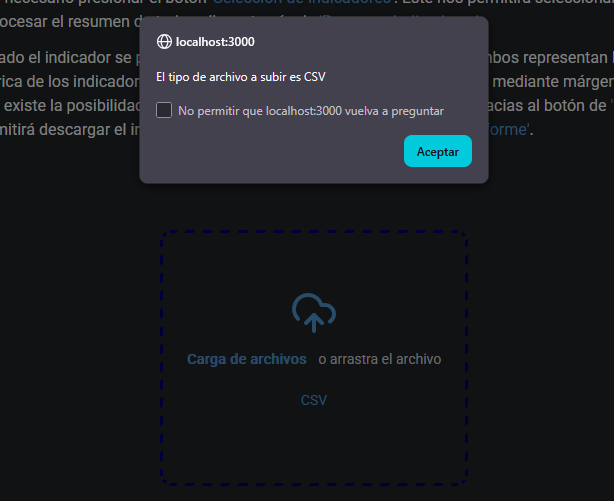
\includegraphics[width=0.8\textwidth]{img/formato.png}
    			\caption{Rechazo de formatos no válidos.}
    			\label{fig:formato}
		\end{figure} 
        
        \item Al superar el límite de 10 archivos cargados, el sistema elimina automáticamente el registro más antiguo (el primero que entró) para alojar el nuevo. Un mensaje por pantalla confirma esta rotación dinámica, garantizando que el usuario siempre disponga de los datos más recientes sin saturar la memoria (Figura \ref{fig:fifo}).
        
        \begin{figure}[hbt!]
    			\centering
    			
\includegraphics[width=0.8\textwidth]{img/fifo.png}
    			\caption{Gestión de la cola \textit{FIFO}.}
    			\label{fig:fifo}
		\end{figure}
    \end{enumerate}
\end{itemize}


\subsubsection{Validación de Estructura: Control de Nomenclatura de Columnas}

Cada indicador clínico de la \textit{SEMICYUC} requiere variables específicas. El sistema debe validar que el archivo cargado contiene la información necesaria para realizar los cálculos matemáticos.

\begin{itemize}
    \item \textbf{Objetivo de la prueba:} Garantizar que el motor de procesamiento detecta la ausencia de columnas obligatorias y detiene la ejecución antes de generar un error de sistema.
    \item \textbf{Ejecución y Resultado:} Se procedió a la carga de un archivo \textit{CSV} con cabeceras alteradas. Al seleccionar un indicador para su análisis, el sistema detecta la inconsistencia y proyecta un mensaje específico en pantalla indicando: ``Error crítico: Falta la columna ``X'' en ``Archivo''. Esta validación evita resultados nulos o \textit{crashes} inesperados (Figura \ref{fig:columnas}).
\end{itemize}

\begin{figure}[hbt!]
    \centering
    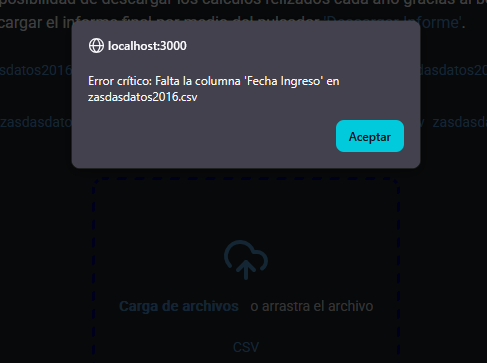
\includegraphics[width=0.8\textwidth]{img/columnas.png}
    \caption{Interrupción controlada del sistema ante la ausencia de columnas requeridas para el cálculo.}
    \label{fig:columnas}
\end{figure}

\subsection{Validación de Transacciones y Gestión de Base de Datos}
La incorporación de la base de datos interactiva exige un nivel de validación superior para garantizar la integridad referencial y clínica del historial médico antes de persistirlo en el disco. El formulario de inserción y edición filtra los datos mediante múltiples capas de seguridad:

\begin{itemize}
    \item \textbf{Tipado y Límites Aritméticos:} El sistema bloquea el guardado si el \textit{Nº de Historia} contiene caracteres no enteros \ref{fig:historia_error}. Asimismo, los parámetros biométricos se evalúan aritméticamente, reemplazando comas por puntos en números decimales y abortando la operación si se detectan valores atípicos absurdos (ej. parámetros con valores superiores a 999).
    
\begin{figure}[hbt!]
    \centering
    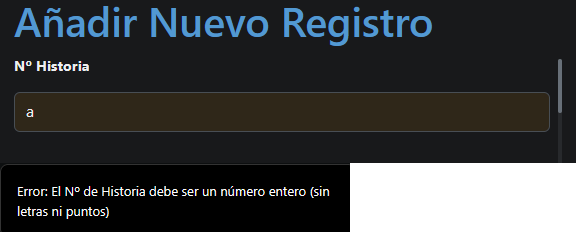
\includegraphics[width=0.8\textwidth]{img/historia_error.png}
    \caption{Número de historia incorrecto.}
    \label{fig:historia_error}
\end{figure}    
    
    \item \textbf{Coherencia Cronológica:} Se emplean algoritmos para evitar imposibilidades clínicas. El sistema asegura que las fechas existan en el calendario (rechazando entradas como ``345/12/2026'') y verifica mediante lógica relacional que la fecha de \textit{Alta} no sea anterior a la de \textit{Ingreso} \ref{fig:fechas_error}, o que el inicio de la Nutrición Enteral (\textit{NE}) ocurra dentro de los márgenes de estancia en la unidad.
    
\begin{figure}[hbt!]
    \centering
    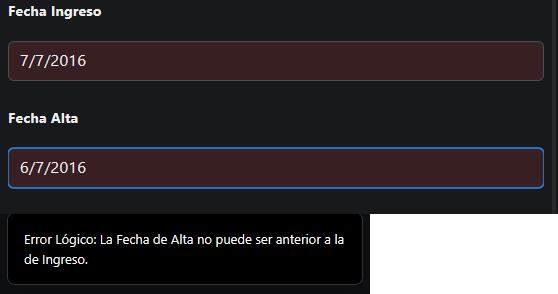
\includegraphics[width=0.8\textwidth]{img/fechas_error.png}
    \caption{Fechas introducidas erróneas.}
    \label{fig:fechas_error}
\end{figure}
    
    \item \textbf{Normalización y Limpieza de Cadenas:} Antes de inyectar texto a \textit{PostgreSQL}, el sistema descompone los caracteres, elimina tildes, purga espacios en blanco residuales y capitaliza la primera letra de cada palabra, asegurando que búsquedas posteriores no fallen por errores tipográficos de los facultativos \ref{fig:cadenas_error}.
    
\begin{figure}[hbt!]
    \centering
    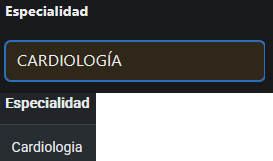
\includegraphics[width=0.8\textwidth]{img/cadenas_error.png}
    \caption{Cadena de texto corregida.}
    \label{fig:cadenas_error}
\end{figure}    
    
    \item \textbf{Auditoría y Anonimización:} Todas las transacciones de escritura, borrado o extracción disparan un registro en una tabla de \textit{Auditoría}, guardando el correo del facultativo y la acción realizada \ref{fig:auditoria_error}. A su vez, se verificó que la rutina de extracción de datos para investigación en formato \textit{ZIP} elimina automáticamente la columna del \textit{Nº de Historia}, garantizando que los archivos exportados cumplan estrictamente con la protección de datos personales.
\end{itemize}

\begin{figure}[hbt!]
    \centering
    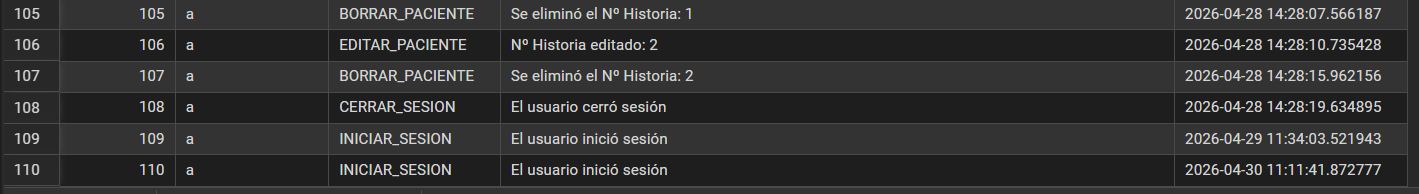
\includegraphics[width=1\textwidth]{img/auditoria_error.png}
    \caption{Registro de auditoria.}
    \label{fig:auditoria_error}
\end{figure} 

\section{Instrucciones para la modificación o mejora del proyecto}
Tal y como se expone en el apartado de ``\textit{Líneas de trabajo futuras}'' de la memoria principal, la arquitectura de este sistema ha sido diseñada bajo principios de escalabilidad y alta cohesión. Esto permite que futuras ampliaciones se integren como nuevos módulos sin necesidad de alterar el código base o reestructurar el motor de renderizado de \textit{Reflex}.

A continuación, se proporcionan las directrices técnicas dirigidas a los futuros desarrolladores encargados de continuar la escalabilidad del sistema hacia un entorno hospitalario integral.

\subsection{Ampliación del Catálogo de Indicadores \textit{SEMICYUC}}
Uno de los pilares de la arquitectura de este proyecto es su escalabilidad. El sistema ha sido diseñado de forma modular, permitiendo la adición de nuevos cálculos clínicos sin necesidad de alterar la lógica central del \textit{software}. Para implementar un nuevo indicador, el desarrollador debe seguir un flujo estandarizado descrito a continuación.

\subsubsection{Fase 1: Creación del Método Base en el \textit{Backend}}
Primero el desarrollador tiene que crear el nuevo método del indicador en el archivo \texttt{Programa.py}, constando de cinco pasos:

\begin{enumerate}
    \item \textbf{Definición del método e inicialización de datos \ref{fig:1_ed}:} 
    El proceso comienza con la declaración de un nuevo método dentro de la clase principal (por ejemplo, \texttt{def nuevo\_indicador(self, ocultar=False):}). Esta primera fase consta de un bloque de código estandarizado que se encarga de iterar sobre los \textit{DataFrames} cargados en memoria (\texttt{self.\_dataframes\_memoria}) y aplicar una limpieza preventiva (como la normalización de cadenas booleanas y la eliminación de columnas duplicadas). En este paso, el desarrollador solo debe modificar el nombre de la función.
    
    	\begin{figure}[hbt!]
    		\centering
    		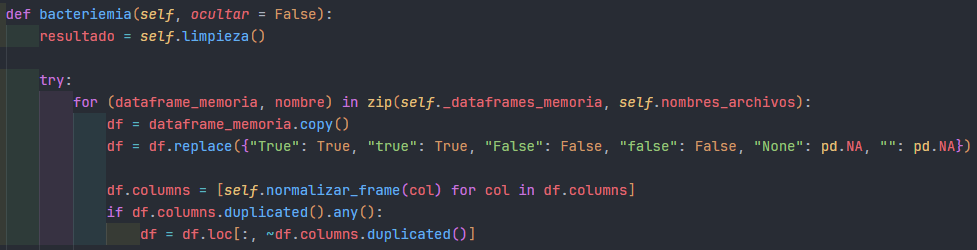
\includegraphics[width=1\textwidth]{img/1_edicion.png}
    		\caption{Definición del Método.}
    		\label{fig:1_ed}
	\end{figure}

    \item \textbf{Validación de variables clínicas (Control de errores) \ref{fig:2_ed}:} 
    Antes de proceder con cualquier operación matemática, es imperativo garantizar la integridad de los datos. Se debe implementar un bloque condicional que verifique si las columnas necesarias para el cálculo (las variables clínicas) existen en el \textit{DataFrame}. En caso de ausencia, el sistema debe levantar una excepción controlada (\texttt{raise ValueError}) informando al usuario de la variable y el archivo donde radica el problema.
    
    \begin{figure}[hbt!]
    		\centering
    		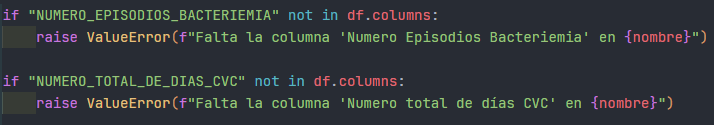
\includegraphics[width=1\textwidth]{img/2_edicion.png}
    		\caption{Validación de Variables Clínicas.}
    		\label{fig:2_ed}
	\end{figure}

    \item \textbf{Lógica de cálculo del indicador \ref{fig:3_ed}:} 
    En esta etapa se programa el núcleo matemático del indicador. Las series de datos extraídas se fuerzan a un formato numérico seguro mediante herramientas como \texttt{pd.to\_numeric} (utilizando la coerción de errores para evitar fallos de ejecución por caracteres anómalos). A continuación, se aplican las operaciones necesarias (sumatorios, medias, ratios por cada 1000 días, etc.) y se añade el valor resultante a la lista global de resultados del método.
    
    \begin{figure}[hbt!]
    		\centering
    		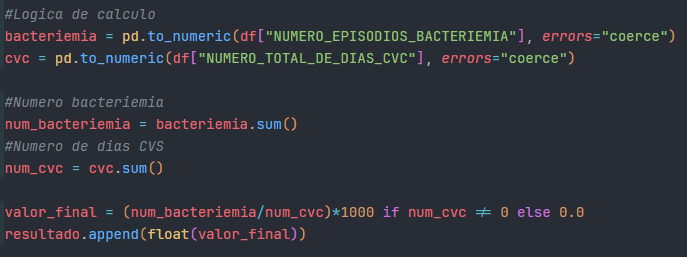
\includegraphics[width=1\textwidth]{img/3_edicion.png}
    		\caption{Cálculo del Indicador.}
    		\label{fig:3_ed}
	\end{figure}

    \item \textbf{Configuración de la exportación de datos (\textit{CSV}) \ref{fig:4_ed}:} 
    Para garantizar la trazabilidad clínica y permitir auditorías posteriores, se debe estructurar la salida de datos. El desarrollador debe crear un diccionario (\texttt{data\_resumen}) que relacione los nombres de las variables con sus valores calculados. Finalmente, se invoca al método de exportación (\texttt{self.csv\_metodo}), pasándole los metadatos necesarios para que la plataforma genere automáticamente el archivo descargable con el desglose de las operaciones.
    
    \begin{figure}[hbt!]
    		\centering
    		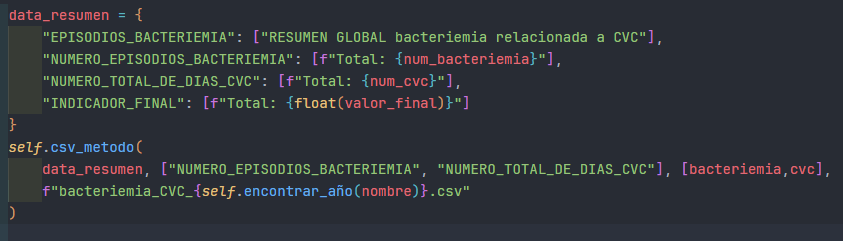
\includegraphics[width=1\textwidth]{img/4_edicion.png}
    		\caption{Exportación de los Datos.}
    		\label{fig:4_ed}
	\end{figure}

    \item \textbf{Renderizado final y documentación clínica \ref{fig:5_ed}:} 
    El último paso consiste en encapsular toda la lógica anterior en un bloque \texttt{try-except}. Si se captura el \texttt{ValueError} definido en el segundo paso, se renderiza una alerta visual en la interfaz del usuario (\texttt{rx.window\_alert}). Si el proceso es exitoso, se concluye llamando al método \texttt{self.final}, al cual se le inyectan los resultados numéricos obtenidos y una cadena de texto descriptiva. Esta descripción contiene la definición clínica formal del indicador y su impacto, siendo el texto que el facultativo leerá en la interfaz \textit{web}.
    
    \begin{figure}[hbt!]
    		\centering
    		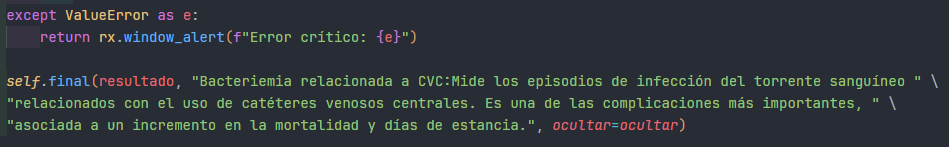
\includegraphics[width=1\textwidth]{img/5_edicion.png}
    		\caption{Renderizado Final.}
    		\label{fig:5_ed}
	\end{figure}
\end{enumerate}

\subsubsection{Fase 2: Integración en el Resumen Global e Informes}
Para que el nuevo indicador forme parte del análisis global y se incluya automáticamente en la exportación masiva y en el informe en formato \textit{PDF}, el desarrollador debe registrarlo en el método encargado de la consolidación de resultados, denominado \texttt{tabla\_resumen}.

Tal y como se establece en la lógica de dicho método, el sistema automatiza la ejecución en bloque de todos los indicadores clínicos. Para integrar el nuevo cálculo en este ciclo, únicamente es necesario modificar dos estructuras de control \ref{fig:7_ed}:

\begin{figure}[hbt!]
    	\centering
    	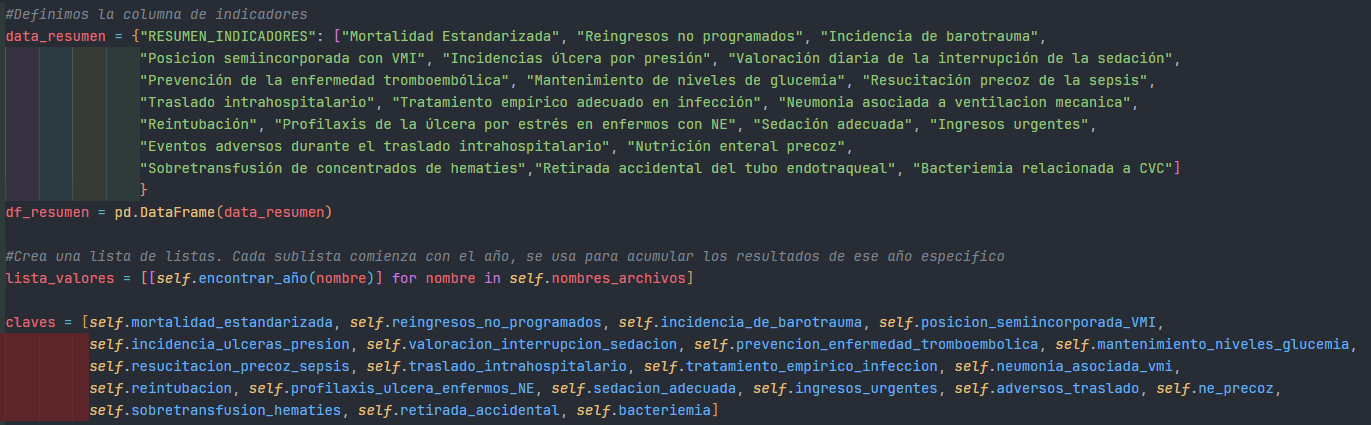
\includegraphics[width=1\textwidth]{img/7_edicion.png}
    	\caption{Inclusión en el Resumen.}
    	\label{fig:7_ed}
\end{figure}

\begin{itemize}
    \item \textbf{Estructura de metadatos (\texttt{data\_resumen}):} Se debe añadir el nombre descriptivo del nuevo indicador al final de la lista asociada a la clave \texttt{``RESUMEN\_INDICADORES''}. Esta cadena de texto será la empleada para identificar la métrica en la tabla visual y en la columna del archivo \textit{CSV} resumen.
    
    \item \textbf{Lista de ejecución (\texttt{claves}):} Se debe incorporar la referencia al método recién creado (por ejemplo, \texttt{self.nuevo\_indicador}) dentro de esta lista. El motor de la aplicación itera sobre esta estructura, invocando y ejecutando cada función de manera silenciosa mediante el parámetro \texttt{ocultar = True}. Esto permite extraer y recopilar sus valores estadísticos en segundo plano sin alterar la interfaz gráfica del facultativo.
\end{itemize}

Con la adición de estos dos únicos elementos, la arquitectura del sistema vincula dinámicamente el nuevo cálculo al flujo principal de la plataforma, garantizando su disponibilidad y trazabilidad en el informe clínico unificado.


\subsubsection{Fase 3: Integración en el Módulo de Análisis Personalizado (Mezcla)}
Si se desea que el nuevo indicador esté disponible en el módulo de análisis combinado (conocido internamente como \texttt{mezcla}), el cual permite al facultativo seleccionar y cruzar diferentes gráficas en una misma vista, es necesario registrar el indicador en dos archivos distintos que separan la lógica del renderizado visual:

\begin{itemize}
    \item \textbf{Mapeo lógico en \texttt{Programa.py}:} Dentro de este archivo, que gestiona el \textit{backend} de la aplicación, se debe localizar el método \texttt{mezcla}. En su interior existe un diccionario denominado \texttt{claves}. El desarrollador debe añadir una nueva entrada donde la clave sea el nombre en texto plano del indicador (ej. \texttt{``Nuevo Indicador Clínico''}) y el valor sea la referencia a su método correspondiente (ej. \texttt{self.nuevo\_indicador}). Este diccionario actúa como un enrutador interno que asocia la selección del usuario con la ejecución del cálculo \ref{fig:8_ed}.
    
    \begin{figure}[hbt!]
    		\centering
    		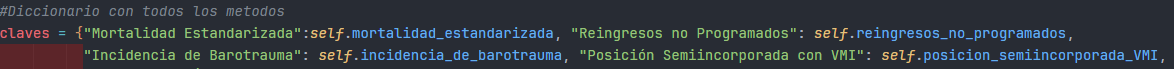
\includegraphics[width=1\textwidth]{img/8_edicion.png}
    		\caption{Método \texttt{mezcla} en \texttt{Programa.py}.}
    		\label{fig:8_ed}
	\end{figure}
    
    \item \textbf{Renderizado en la interfaz gráfica en \texttt{mezcla.py}:} Para que el indicador sea visible y seleccionable por el usuario en el \textit{frontend}, se debe modificar el archivo \texttt{mezcla.py}. Dentro de la estructura que genera los botones de selección, se encuentra un componente iterador \texttt{rx.foreach} \ref{fig:9_ed}. El desarrollador únicamente debe añadir el nombre exacto del indicador (el mismo texto plano utilizado como clave en el paso anterior) a la lista de cadenas de texto que procesa este componente. De este modo, \textit{Reflex} generará automáticamente el elemento visual con los estilos predefinidos de la plataforma.
    
    \begin{figure}[hbt!]
    		\centering
    		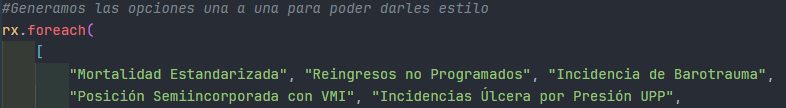
\includegraphics[width=1\textwidth]{img/9_edicion.png}
    		\caption{Método \texttt{mezcla} en \texttt{mezcla.py}.}
    		\label{fig:9_ed}
	\end{figure}
\end{itemize}

Esta separación de responsabilidades entre el mapeo de la lógica (\texttt{Programa.py}) y la generación de la vista (\texttt{mezcla.py}) obedece al patrón de diseño del \textit{framework}, manteniendo el código limpio y facilitando la inyección de nuevos componentes en la interfaz reactiva.


\subsubsection{Fase 4: Accesibilidad Individual en el Menú de Navegación}

Para concluir la integración y permitir que el facultativo pueda ejecutar y visualizar el nuevo indicador de forma aislada, es indispensable vincularlo a la interfaz de usuario principal de la aplicación. Esta acción se lleva a cabo en el archivo encargado de renderizar el menú de opciones del \textit{frontend}, denominado \texttt{seleccion.py}.

Dentro de este archivo, se ubica el contenedor del menú desplegable definido por el componente \texttt{rx.menu.content}. Para incorporar la nueva funcionalidad, el desarrollador debe instanciar un nuevo elemento dentro de este contenedor utilizando \texttt{rx.menu.item}, configurando dos parámetros fundamentales \ref{fig:10_ed}:

\begin{figure}[hbt!]
    	\centering
    	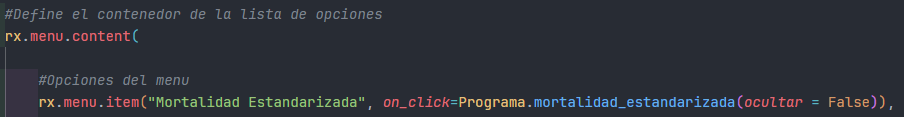
\includegraphics[width=1\textwidth]{img/10_edicion.png}
    	\caption{Método \texttt{seleccion} en \texttt{seleccion.py}.}
    	\label{fig:10_ed}
\end{figure}

\begin{itemize}
    \item \textbf{Etiqueta visual:} Una cadena de texto con el nombre clínico del indicador (por ejemplo, \texttt{"Nuevo Indicador"}), que servirá como la opción visible y descriptiva para el usuario.
    \item \textbf{Evento de invocación (\texttt{on\_click}):} Se debe enlazar este disparador de eventos al método correspondiente alojado en la clase principal del \textit{backend}. Para ello, se pasa como argumento la llamada directa a la función (ej. \texttt{Programa.nuevo\_indicador(ocultar = False)}). 
\end{itemize}

Es crucial mantener el parámetro \texttt{ocultar = False} en esta llamada. A diferencia de la ejecución masiva en segundo plano vista en los resúmenes globales, este booleano instruye al motor de la aplicación para que procese los datos y, acto seguido, renderice las gráficas y estadísticas en la pantalla principal del usuario.

Con la adición de este botón, el nuevo indicador queda plenamente integrado en todas las capas de la arquitectura del \textit{software}: motor de cálculo interno, resúmenes globales, vistas combinadas y consulta individual, dando por finalizado el proceso de extensión de la herramienta.

\subsubsection{Fase 5 (Opcional): Renderizado de Gráficos}
En caso de que el nuevo indicador requiera un análisis temporal evolutivo a través de la interfaz visual (generado mediante la librería \textit{Matplotlib}), es altamente recomendable configurar la semántica de colores de su gráfica. Para ello, el desarrollador debe dirigirse al método \texttt{grafico} alojado en el archivo \texttt{Programa.py} \ref{fig:6_ed} y añadir el nombre de la variable al diccionario de control interno denominado \texttt{claves} .

\begin{figure}[hbt!]
    	\centering
    	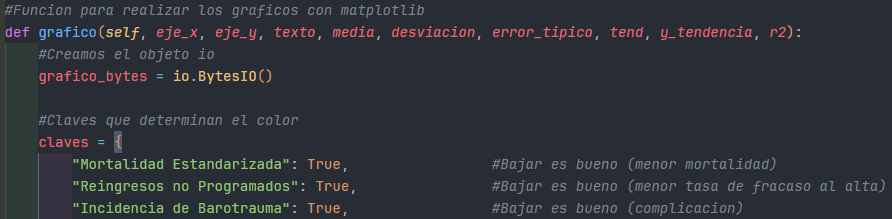
\includegraphics[width=1\textwidth]{img/6_edicion.png}
    	\caption{Claves para su Renderizado.}
    	\label{fig:6_ed}
\end{figure}

Este diccionario asocia la cadena de texto identificativa del indicador con un valor booleano (\texttt{True} o \texttt{False}) que define la lógica de renderizado de la línea de tendencia:

\begin{itemize}
    \item \textbf{Valor \texttt{True} (Tendencia descendente favorable):} Se asigna a aquellos indicadores clínicos donde una reducción en su valor numérico absoluto representa una mejora en la calidad asistencial. Bajo esta configuración, el sistema pintará automáticamente los descensos en la gráfica de color verde (positivo) y los incrementos en color rojo (alerta).
    
    \item \textbf{Valor \texttt{False} (Tendencia ascendente favorable):} Se reserva para indicadores donde un incremento temporal denota un escenario clínico positivo. En este caso, la lógica de colores se invierte en el renderizado de la imagen final.
\end{itemize}

\subsection{Mantenimiento, Escalabilidad y Migración de la Base de Datos}
En este apartado se detalla el protocolo técnico estandarizado para la adición de nuevas variables clínicas al sistema. Dada la arquitectura basada en \textit{Reflex} y \textit{PostgreSQL}, es imperativo seguir un flujo de trabajo riguroso que garantice la integridad referencial de los datos históricos y la correcta asimilación de los cambios estructurales tanto en la interfaz gráfica como en el despliegue mediante \textit{Docker}. El procedimiento se articula en las tres fases consecutivas descritas a continuación.

\subsubsection{Fase 1: Modificación del Esquema Lógico del Modelo (\texttt{Modelo.py})}
El primer paso consiste en declarar la nueva variable dentro de la clase \texttt{Registro} alojada en el archivo \texttt{Modelo.py} \ref{fig:11_ed}, la cual hereda de \texttt{rx.Model} y actúa como el mapeador objeto-relacional (\textit{ORM}).

\begin{figure}[hbt!]
    	\centering
    	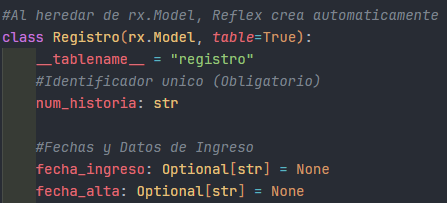
\includegraphics[width=1\textwidth]{img/11_edicion.png}
    	\caption{Tabla \texttt{Registro} en el archivo \texttt{Modelo.py}.}
    	\label{fig:11_ed}
\end{figure}

La nomenclatura del nuevo campo debe ajustarse estrictamente a la convención \texttt{snake\_case}\footnote{Convención de escritura que consiste en escribir palabras compuestas en minúsculas y separarlas mediante un guion bajo (\_) en lugar de usar espacios.}. Asimismo, es un requisito arquitectónico ineludible que la variable sea declarada mediante el tipado \texttt{Optional} y se le asigne el valor por defecto \texttt{None}. Esta práctica asegura la retrocompatibilidad del sistema, permitiendo que las consultas a los registros históricos (previos a la creación de este nuevo campo) no generen excepciones por ausencia de datos estructurales.

\subsubsection{Fase 2: Configuración del Motor Lógico e Interfaz (\texttt{BBDD.py})}
Una vez actualizado el modelo físico de la base de datos, es necesario modificar el motor lógico para que el \textit{frontend} procese adecuadamente la variable. Esto se logra alterando las listas maestras del Estado (\textit{State}) de \textit{Reflex}.

\paragraph{Mapeo de Variables y Sincronización de Índices:}La nueva variable debe ser añadida obligatoriamente en tres listas principales ubicadas en la clase \texttt{BBDD} del archivo \texttt{BBDD.py}. Para evitar desajustes en la renderización de las celdas de la tabla de registros, el nuevo campo \textbf{debe ocupar exactamente la misma posición relativa (índice)} en todas ellas:

\begin{enumerate}
    \item \texttt{cabeceras} \ref{fig:12_ed}: Representa el nombre exacto de la columna tal y como consta en la base de datos (formato \texttt{snake\_case}).
    
	\begin{figure}[hbt!]
    		\centering
    		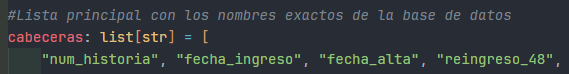
\includegraphics[width=1\textwidth]{img/12_edicion.png}
    		\caption{Lista \texttt{cabeceras}.}
    		\label{fig:12_ed}
	\end{figure}    
    
    \item \texttt{cabeceras\_display} \ref{fig:13_ed}: Representa el nombre amigable o etiqueta visual que consumirá la interfaz gráfica (utilizando \textit{Title Case}\footnote{La mayúscula inicial o mayúscula inicial es un estilo de mayúsculas utilizado para representar los títulos de obras publicadas o de arte en inglés.} y respetando la acentuación ortográfica).
    
	\begin{figure}[hbt!]
    		\centering
    		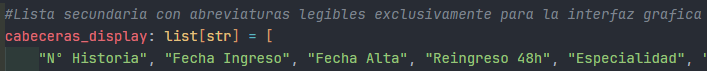
\includegraphics[width=1\textwidth]{img/13_edicion.png}
    		\caption{Lista \texttt{cabeceras\_display}.}
    		\label{fig:13_ed}
	\end{figure}  
    
    \item \texttt{cabeceras\_exportacion} \ref{fig:14_ed}: Define la cabecera exigida por los \textit{scripts} analíticos construidos sobre \textit{Pandas} al generar archivos \textit{CSV} o volcados a unidades extraíbles. Son los nombres utilizados para el cálculo en el archivo \texttt{Programa.py}.
    
	\begin{figure}[hbt!]
    		\centering
    		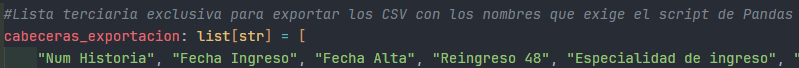
\includegraphics[width=1\textwidth]{img/14_edicion.png}
    		\caption{Lista \texttt{cabeceras\_exportacion}.}
    		\label{fig:14_ed}
	\end{figure}    
    
\end{enumerate}

Seguidamente, la variable utilizada en la lista \texttt{cabeceras\_display} debe ser incluida en la lista \texttt{orden\_formulario} \ref{fig:15_ed}, lo cual dictará su posición visual exacta en el formulario modal dinámico de inserción y edición de pacientes.

\begin{figure}[hbt!]
    	\centering
    	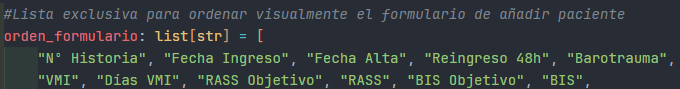
\includegraphics[width=1\textwidth]{img/15_edicion.png}
    	\caption{Lista \texttt{orden\_formulario}.}
    	\label{fig:15_ed}
\end{figure}

\paragraph{Clasificación de Tipos para Renderizado Dinámico:}Para que la función del \textit{frontend} denominada \texttt{renderizar\_campo\_formulario} sea capaz de pintar el componente adecuado (\textit{input} de texto, numérico o \textit{select}) y valide correctamente las restricciones, el parámetro debe clasificarse (utilizando la misma cadena de texto que en la lista \texttt{cabeceras\_display}) incluyéndolo en una de las siguientes listas de control de tipos. Si la variable es texto libre, no es necesario incluirla en ninguna de estas listas; el sistema generará un input de texto genérico por defecto:

\begin{itemize}
	\item \texttt{campos\_display\_fecha} o \texttt{campos\_display\_fecha\_multiple} \ref{fig:16_ed}: Utilizadas para gestionar la inclusión de fechas o conjunto de fechas.
	\begin{figure}[hbt!]
    		\centering
    		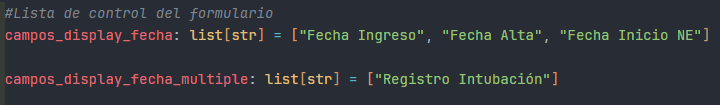
\includegraphics[width=1\textwidth]{img/16_edicion.png}
    		\caption{Lista \texttt{campos\_display\_fecha} y \texttt{campos\_display\_fecha\_multiple}.}
    		\label{fig:16_ed}
	\end{figure}
	
    \item \texttt{campos\_display\_numerico} \ref{fig:17_ed}: Contiene todos los campos que se basan en cifras numéricas.
    \begin{figure}[hbt!]
    		\centering
    		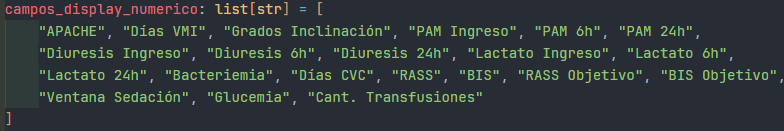
\includegraphics[width=1\textwidth]{img/17_edicion.png}
    		\caption{Lista \texttt{campos\_display\_numerico}.}
    		\label{fig:17_ed}
	\end{figure}
    
    \item \texttt{campos\_display\_booleano} \ref{fig:18_ed}: Almacena los registros booleanos.
    \begin{figure}[hbt!]
    		\centering
    		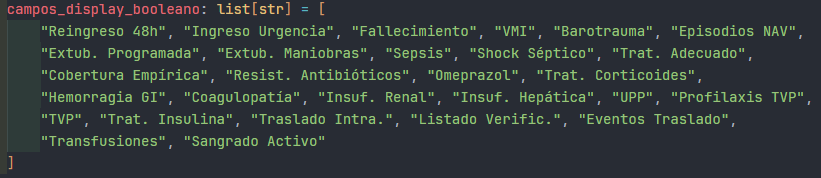
\includegraphics[width=1\textwidth]{img/18_edicion.png}
    		\caption{Lista \texttt{campos\_display\_booleano}.}
    		\label{fig:18_ed}
	\end{figure}
    
\end{itemize}

\paragraph{Restricciones Lógicas en el Procesamiento de Datos:}Finalmente, en el método \texttt{guardar\_nuevo\_paciente}, se deben añadir las comprobaciones lógicas oportunas. Por defecto el sistema valida el tipo numérico del número de historia \ref{fig:19_ed}, la validez y sentido lógico de las fechas, comprueba el tipo de las variables numéricas y las limita a no superar el máximo de 1000 unidades. Al añadir nuevas columnas, será decisión del desarrollador incluir las verificaciones que considere oportunas.

\begin{figure}[hbt!]
    	\centering
    	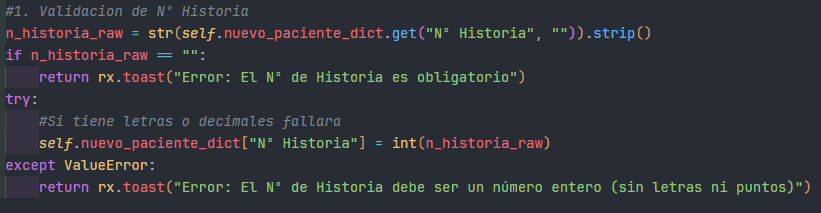
\includegraphics[width=1\textwidth]{img/19_edicion.png}
    	\caption{Verificación \texttt{Nº Historia}.}
    	\label{fig:19_ed}
\end{figure}

\subsubsection{Fase 3: Ciclo de Migración Estructural Segura de Datos (\textit{Alembic} y \textit{Docker})}
El último eslabón del mantenimiento implica alterar el esquema físico de \textit{PostgreSQL}. Para ello, se utiliza el motor de migraciones \textit{Alembic} (integrado nativamente en \textit{Reflex}), el cual permite inyectar columnas en caliente sin provocar la pérdida de los registros clínicos ya consolidados en el sistema.

Para el procedimiento de despliegue es necesario abrir la terminal del entorno de desarrollo (en el directorio raíz) y ejecutar la siguiente secuencia de comandos:

\begin{enumerate}
    \item \textbf{Generación del \textit{script} automático de migración temporal:} El sistema compara el modelo lógico definido en \textit{Python} con el esquema vivo de la base de datos para registrar las diferencias.

\texttt{reflex db makemigrations -{}-message ``Agregada nueva variable clinica''}


    \item \textbf{Aplicación física de la migración:} Se consolida el cambio, inyectando la nueva columna en el esquema final de la tabla de \textit{PostgreSQL}.
    
\texttt{reflex db migrate}


    \item \textbf{Reconstrucción y despliegue del contenedor:} Se asimilan los nuevos archivos de migración a nivel de infraestructura reiniciando los servicios orquestados.
    
\texttt{docker-compose up -d -{}-build}
\end{enumerate}

\textbf{\textit{Nota técnica de integridad referencial:}} Al ejecutar exitosamente el ciclo de migración, los registros antiguos (pacientes ingresados con anterioridad al parche) inicializarán automáticamente esta nueva columna con un valor nulo (\texttt{NULL} a nivel de base de datos, mapeado como \texttt{None} en \textit{Python}). Este comportamiento por diseño garantiza la absoluta coherencia de los datos y previene caídas del sistema por desajustes posicionales durante la lectura.

\subsection{Transición a Ingesta Automatizada (Integración con ICCA)}
Sustituir el actual sistema de carga manual de registro en la \textit{BBDD} por una conexión en tiempo real con el sistema \textit{ICCA}, el desarrollador deberá modificar el módulo de ingesta de datos respetando la arquitectura de eventos de \textit{Reflex}.
\begin{itemize}
    \item \textbf{Directriz técnica:} Se debe implementar un cliente de interoperabilidad basado en estándares internacionales de salud (\textit{HL7} \cite{hl7} o \textit{FHIR}). El programador deberá reemplazar la función actual de ingesta por una tarea en segundo plano (\textit{Background Task}\footnote{Proceso o rutina que se ejecuta sin necesidad de la interacción directa del usuario, permitiendo que la aplicación principal siga funcionando sin interrupciones.}) que realice peticiones \textit{API REST} periódicas (ej. mediante la librería \texttt{requests} o \texttt{httpx} en \textit{Python}) al servidor \textit{ICCA}, inyectando los datos estructurados directamente en el \textit{DataFrame} del estado global de la aplicación.
\end{itemize}

\subsection{Implementación de Modelos de \textit{Machine Learning}}

La integración de modelos predictivos de la librería \textit{Scikit-Learn} requerirá un manejo cuidadoso de los recursos del servidor para no bloquear la interfaz de usuario durante el procesamiento algorítmico intensivo.
\begin{itemize}
    \item \textbf{Directriz técnica:} El entrenamiento y la inferencia de los modelos (ej. árboles de decisión o regresiones logísticas para predecir alteraciones en los indicadores) deben programarse utilizando la asincronía nativa de \textit{Python} (\texttt{async/await} \cite{await}). De este modo, mientras el modelo matemático calcula el riesgo del paciente, la interfaz gráfica (\textit{Frontend}) seguirá respondiendo a las interacciones táctiles del facultativo sin sufrir bloqueos (\textit{Thread blocking}\footnote{Concepto de programación concurrente donde un hilo de ejecución se detiene y queda en espera (``bloqueado'') hasta que se cumpla una condición específica}).
\end{itemize}

\section{Vías de Implantación en la Infraestructura Hospitalaria}
La arquitectura del sistema ha sido concebida bajo el paradigma de contenerización (\textit{Docker}), lo que otorga a la plataforma un alto grado de flexibilidad, portabilidad y modularidad. Esta decisión tecnológica permite que la herramienta se integre en la \textit{intranet} del hospital adaptándose a las políticas de seguridad y a los recursos del departamento de informática. Para su paso a producción, se contemplan dos vías principales de implantación operativa:

\subsection{Vía A: Despliegue Íntegro sobre Infraestructura Dedicada}
Este escenario es el más directo y asume la provisión de una \textbf{Máquina Virtual (\textit{VM}\footnote{Entorno informático basado en software que emula un ordenador físico, ejecutando su propio sistema operativo y aplicaciones de forma aislada.})} limpia y dedicada exclusivamente al proyecto por parte de los servicios informáticos del hospital. Bajo este enfoque, se replica exactamente la arquitectura orquestada y validada durante la fase de desarrollo.

\begin{itemize}
    \item \textbf{Despliegue Técnico:} Se ejecuta el archivo \texttt{docker-compose.yml} en su totalidad, levantando de forma simultánea e interconectada el contenedor de la aplicación \textit{web} (\textit{Reflex}) y el contenedor del motor relacional (\textit{PostgreSQL}), asegurando la creación de los volúmenes de persistencia (\texttt{pgdata}) en la propia máquina.
    \item \textbf{Acceso Clínico:} El departamento técnico asigna una \textit{IP} estática a la \textit{VM} dentro de la red local. Los facultativos de la \textit{URCCPQ} acceden al sistema introduciendo dicha dirección en los navegadores de sus puestos de trabajo (por ejemplo, \texttt{http://10.X.X.X:3000}), garantizando un entorno autónomo, aislado y de baja latencia.
\end{itemize}

\subsection{Vía B: Integración Desacoplada con la Base de Datos Corporativa}
En entornos institucionales con protocolos de centralización de datos estrictos, es frecuente que el hospital exija alojar toda la información clínica en su propio clúster de servidores \textit{PostgreSQL} preexistente para unificar las copias de seguridad (\textit{backups}) y el cumplimiento normativo. La arquitectura del siguiente \textit{GitHub}: \href{https://github.com/ngg1017/TFG-2026-Nicolas-Garcia-Gomez-Produccion}{TFG-2026-Nicolas-Garcia-Gomez-Produccion}. Permite un desacoplamiento nativo del despliegue local satisfaciendo este requisito.

\begin{itemize}
    \item \textbf{Adaptación de la Orquestación:} Se excluye el servicio de base de datos local del archivo \texttt{docker-compose.yml}, de forma que la \textit{VM} del proyecto únicamente aloje y procese el contenedor correspondiente al \textit{frontend} y \textit{backend} de la aplicación.
    \item \textbf{Enrutamiento de Datos:} La persistencia se redirige modificando de forma segura el archivo oculto de credenciales (\texttt{.env}). Se actualiza la variable \texttt{DATABASE\_URL} para inyectar la cadena de conexión proporcionada por el hospital. De este modo, la aplicación se comunica de forma transparente a través de la \textit{intranet} con el servidor corporativo, delegando la gestión física del almacenamiento a la infraestructura central de la institución médica.
\end{itemize}